\chapter{Tests and results}
\label{ch:tests}

In this chapter the tests made in the simulator to test the behavior of the proposed algorithm will be explained, as well as the results.

\section{Test setup}

To test how the algorithm behaves in real life traffic scenarios, a 16 hour simulation will be done. 100000 cars will be randomly generated, their start and ending points can only be one of the 26 existing intersections, and they can chose any path combining the 58 available segments. The car maximum speed is between 80 and 120.

The test will be carried on 11 separated simulations, each of one containing a different percentage of cars using the proposed algorithm, from 0\% to 100\%. To get more interesting results, \textit{the same cars} will be used in every simulation, that's the same origin, destiny, time of appearance, and maximum speed. The only thing that will change is that from those initial cars, a subset will be chosen and their routing algorithm will change to the smart algorithm.

The Figure \ref{graph} shows how the graph has been constructed, the weights are the distance in kilometers and the maximum speed between those two nodes. Also in Figure \ref{map} we can see where the physical intersections are.

\begin{figure}[!ht]
  \centering
  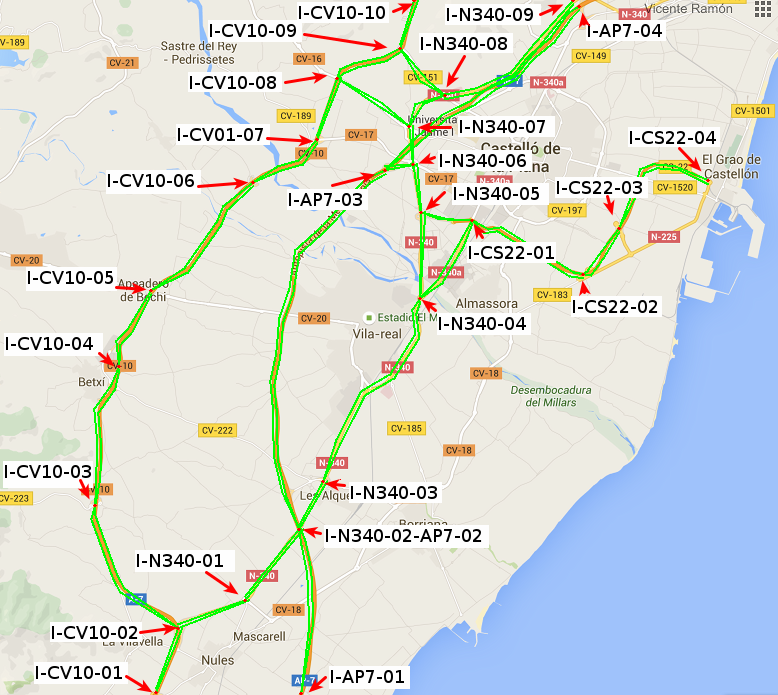
\includegraphics[scale=0.4]{images/map.png} 
  \caption{Road network map}
  \label{map}
\end{figure}

\begin{figure}[!ht]
  \centering
  \includegraphics[scale=0.4]{images/graph.png} 
  \caption{Road network graph}
  \label{graph}
\end{figure}

\section{Results}

The goal of this tests is to show how the smart cars behave in a dynamic environment. To see how the percentage of them affects the system, the data of all the segments have been retrieved. This data contains the number of cars, the service level, the maximum speed for that segment and the current speed.

The current speed is dependent of the service level of the segment and is the maximum allowed speed at that point in time. Figure \ref{traffic} (a bigger version of this figure can be found at Figure \ref{ap:traffic}) shows a plot for 16 hours for one of the most demanding segments. It is easy to see that the more cars there are in the segment, the slower the current speed. In this segment a extreme situation is never reached, but gives a good overview of how to used the output data from the MAS.

With this data, the best results we can take is the average current speed for all segments on a given simulation, and we can compare the 11 simulations to see how the system has performed. This will give us a very good idea of how the system becomes more stable and efficient the more smart cars there are. The results have been plotted in Figure \ref{vcurrent} (a bigger version of this figure can be found at Figure \ref{ap:vcurrent})  and, as expected, the system behaves better when we increase the percentage of smartcars.

The peak at 8:00 is caused because prior to that there are no cars on the simulator, so they can move freely and at maximum speed at first. After that we can see a low speed area when the event manager starts adds all the agents, because all the agents are added in valid intersections and the system has not been stabilized some segments start to lower its service level. After that the system stabilizes with a low number of vehicles per segment, allowing full speed on most of them. And then, when cars are added the system fully stabilizes and smartcars start to dynamically adjust their routes. The average number of cars per segment can be seen in Figure \ref{numCars} (a bigger version of this figure can be found at Figure \ref{ap:numCars}) .

We can see that in both Figures, when the system does not have any smart node, it behaves really poorly. Its average speed as seen in Figure \ref{vcurrent} is way lower than any other case. It is surprising that even with a 10\% of the cars being aware of the traffic, the average speed has an improvement of 3 km/h. This is also obvious in the average number of cars per segment, Figure \ref{numCars}, when we can see that when there is a raise on the proportion of smartcars, there are less cars on the network. That is due to them reaching faster their destinations.

\begin{figure}[!ht]
\hspace{-1.5cm}% Move it slightly to the left
  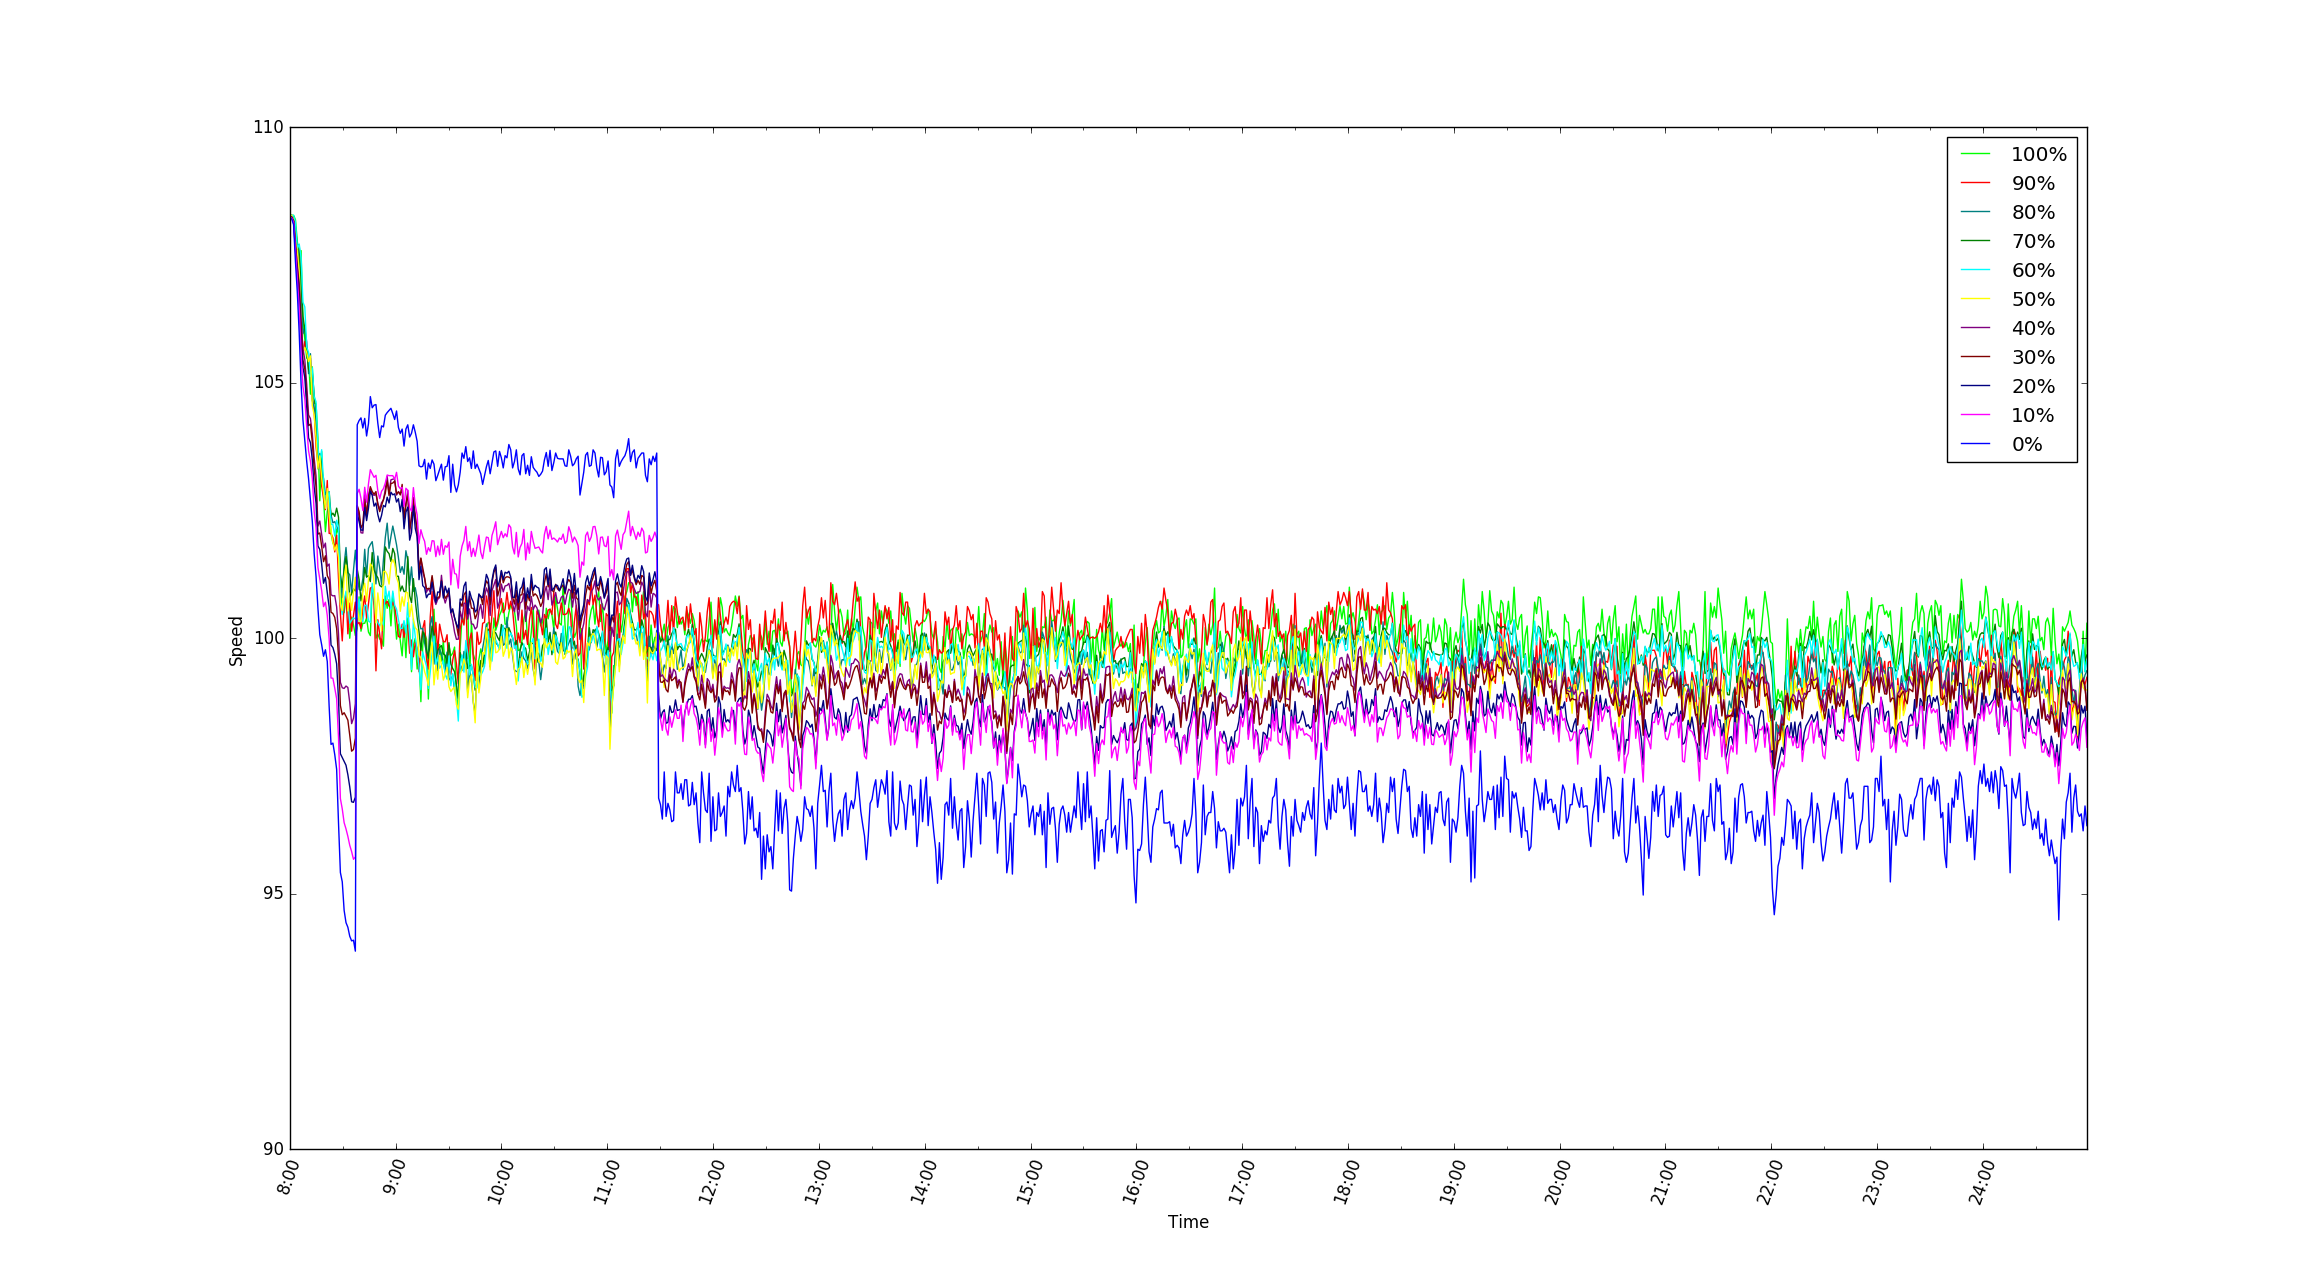
\includegraphics[scale=0.3]{images/Speed.png}
  \caption{Results for the mean current velocity speed}
  \label{vcurrent}
\end{figure}

\begin{figure}[!ht]
\hspace{-1.5cm}% Move it slightly to the left
  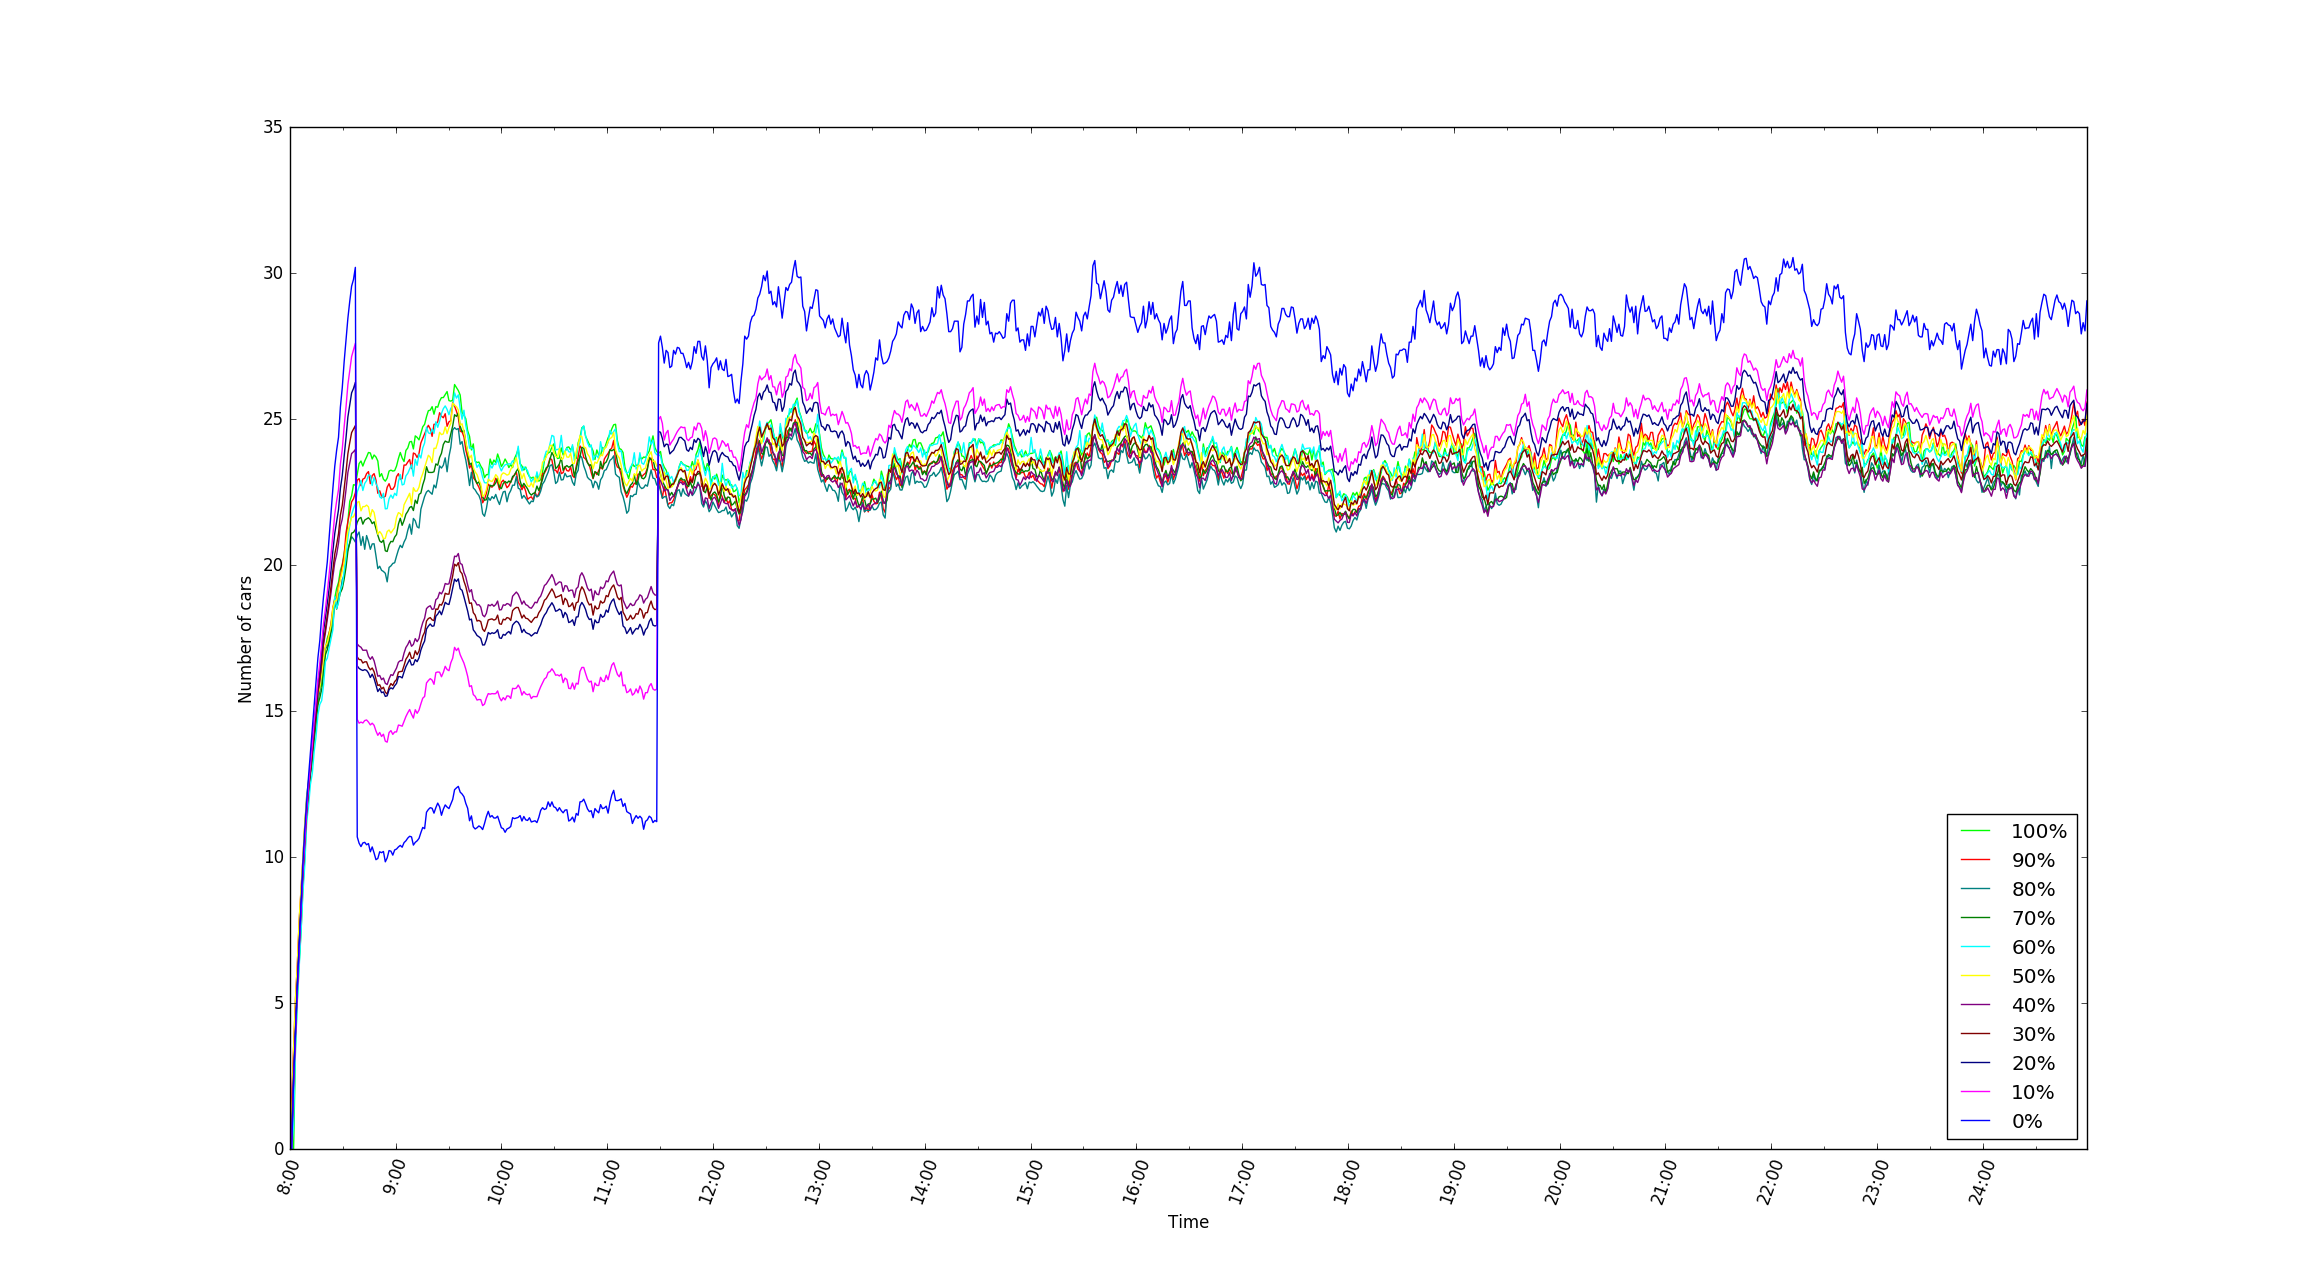
\includegraphics[scale=0.3]{images/Num_cars.png}
  \caption{Results for the mean current number of cars}
  \label{numCars}
\end{figure}

\begin{figure}[!ht]
\
  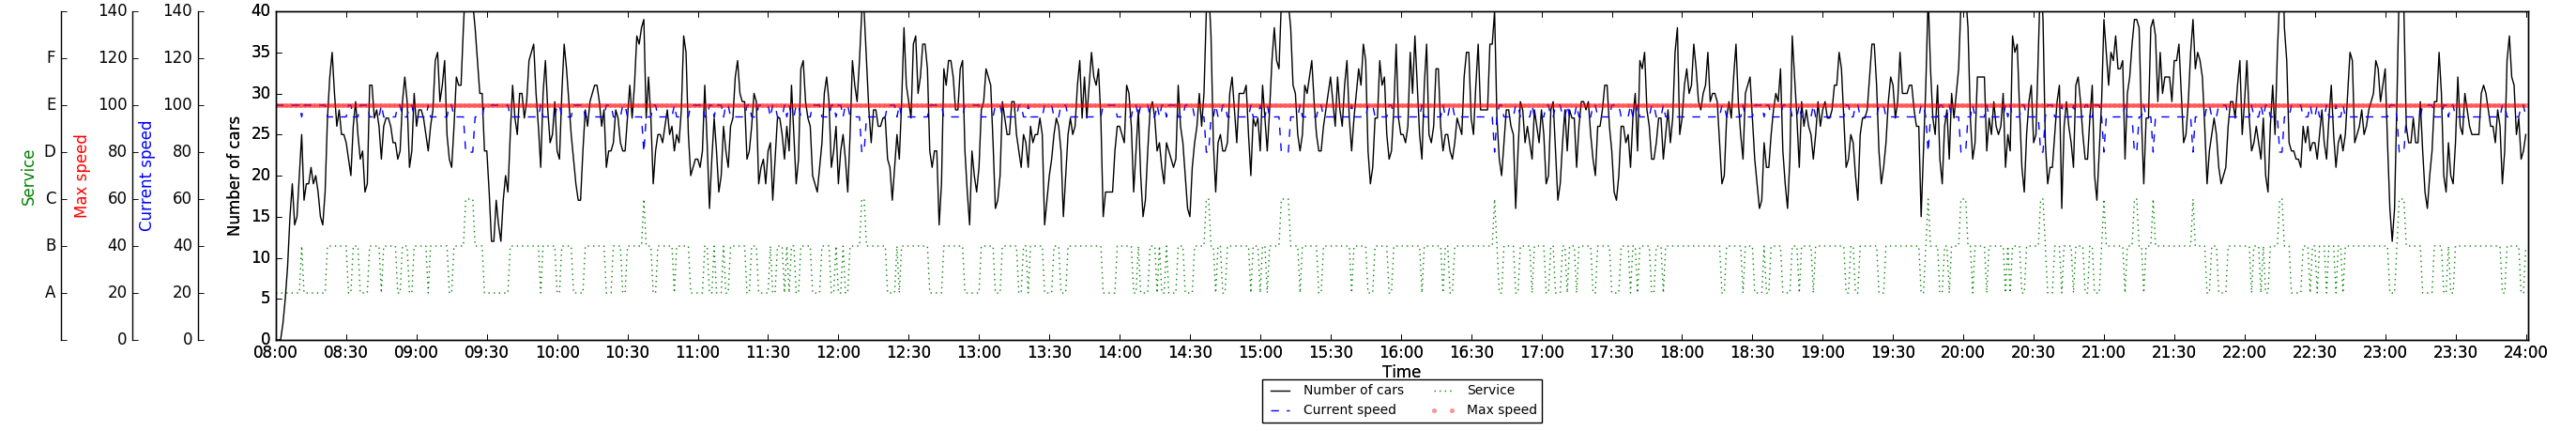
\includegraphics[scale=0.2]{images/cs2201.png}
  \caption{Traffic on the segment CS-22-01}
  \label{traffic}
\end{figure}